\section{The \tool{} Approach}\label{sec:approach}

A slice helps a developer only as lines of their own program. The \tool{} approach computes the QDG slice of
Section~\ref{sec:core} statically on the source of a Qiskit program~\cite{javadi2024qiskit} or an OpenQASM~2
circuit, and shows it as source lines, the loop iterations that put each line in the slice, the classical lines
that compute its qubits and angles, and a profile of each qubit. We implement the approach as a tool,
\tool{}. This section describes the approach, whose steps Fig.~\ref{fig:overview} shows, and the evidence that
the implementation computes the slices that Section~\ref{sec:core} defines.

\begin{figure*}[t]
  \centering
  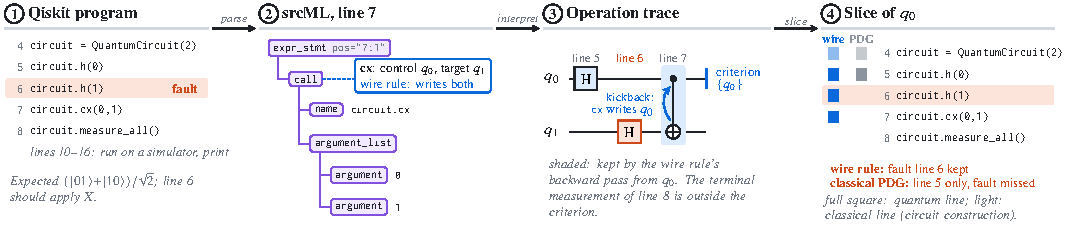
\includegraphics[width=\textwidth]{figures/fig_overview.pdf}
  \caption{The paper at a glance. Top, the method: what a slice must keep, the rule that produces it, the study
  that measures the alternatives and the implications. Bottom, the \tool{} approach: two front ends, the parts
  taken from srcML and srcSlice, the quantum extensions E1 to E5, and what a developer is shown. The dashed arrow
  marks that the rule the study confirms is the rule \tool{} runs.}
  \label{fig:overview}
\end{figure*}

\subsection{Why build on srcML and srcSlice}
Four properties of srcML and srcSlice matter for a slicer whose output a developer reads. First, srcML parses a file as
text and never compiles it~\cite{collard2011lightweight}, so the approach slices programs that cannot be run,
such as fragments, programs written for earlier Qiskit releases and programs from untrusted sources, and it needs
neither a simulator nor quantum hardware. Second, srcML keeps every character of the source and the position of
every element and converts back to source without loss~\cite{collard2011lightweight}, so a slice is shown on the
developer's own text. Third, srcML marks up its languages with one vocabulary of elements~\cite{collard2013srcml},
and a markup for OpenQASM has been specified~\cite{behler2024supporting}, so the classical and quantum parts of a
program can share one representation~\cite{behler2025static}. Fourth, srcSlice's slicing from profiles,
without a dependence graph, scales to large systems, as Section~\ref{sec:related} describes.

What neither tool provides is the quantum meaning of a program. srcML marks a Qiskit program up as Python, so
\texttt{qc.cx(qubit, qubit + 1)} is a call with two argument expressions, and to srcSlice the circuit \texttt{qc} is
one variable used on every gate line. srcSlice therefore knows which variables reach which argument of which call,
but not which qubits a gate acts on, and its slice of \texttt{qc} is the whole circuit. The approach adds this
meaning in five extensions, E1 to E5 in Fig.~\ref{fig:overview}.

\subsection{From source to slices}
\paragraph*{E1, quantum roles of calls}
A table of \numToolGateTable{} Qiskit instruction methods, including those of earlier releases, records which
arguments of each are qubits, classical bits and angles, and which leading qubits are controls. It turns a call in
the srcML tree into an operation on qubit operands. In OpenQASM the syntax states these roles, and in Qiskit the
table supplies them.

\paragraph*{E2, the operation trace}
A static interpretation of the srcML tree turns the program into the circuit it builds, as a trace of operations,
each tagged with its source line and with the iteration of every loop that encloses it. Qiskit computes qubit
indices, sizes and angles in Python, so the interpretation evaluates the program's expressions over the values it
can know, unrolls loops, inlines functions and follows the conditioned gates, branches and loops of the circuit as
Section~\ref{sec:loops} describes. Where a value cannot be known statically, it over-approximates. An unknown qubit
index acts on every qubit it may denote, every branch of an unknown condition is interpreted, and a loop of unknown
length is handled as Section~\ref{sec:loops} describes, with at most \numToolMaxCopies{} copies of its body. Each of these is reported to the
developer, and a circuit passed to code the interpretation does not model is reported as not traced.

\paragraph*{E3, the write-all slice}
srcSlice reads a statement as defining the variables it assigns and using the others, so to srcSlice
\texttt{qc.cx(a, b)} defines nothing. For qubits, the approach reads it by the write-all rule of
Definition~\ref{def:writeall} instead, so a gate defines and uses all its qubits, a measurement defines its bit, and
a conditioned operation uses the bits its condition reads. Like srcSlice, \tool{} builds no dependence graph. The QDG
specifies the slice, and \tool{} computes it with the backward pass of Theorem~\ref{thm:sound} over the trace, in
time linear in the trace. An operation that may act on several qubits adds all of them to the needed set, so the
over-approximations of E2 can only enlarge a slice. A forward pass gives the forward slice of
Proposition~\ref{prop:dual}. For large circuits, the implementation also carries a set of criterion qubits on every
needed location, which gives the backward slice of every qubit in a single pass.

\paragraph*{E4, classical lines}
The lines that compute a slice's qubits, angles, conditions and loop ranges come from srcSlice's profiles. The
start lines are the slice's quantum lines and the headers of the loops, conditions and \texttt{with} blocks that
enclose them. The profiles used on a start line are followed backward to their definitions, to the variables that
flow into them and, for a function parameter, to the arguments passed in its place. srcSlice is run with a patch
that adds Python and two fixes that building \tool{} exposed, for uses inside a subscript, as in \texttt{q[a]},
which is how Qiskit names qubits and C indexes arrays, and for module variables read inside a function. The patch applies to the public srcSlice and is in the
replication package with its regression tests.

\paragraph*{E5, qubit profiles}
The profile of Definition~\ref{def:profile} comes from one backward and one forward pass over the trace and from
the srcML of the gate calls on the qubit.

\subsection{Two front ends}
The approach reads Qiskit programs, the language of the real programs of Bugs4Q and LintQ's
corpus~\cite{zhao2023bugs4q, paltenghi2024lintq}, and OpenQASM~2 circuits, the format that Qiskit exports and the
benchmark suites ship in. In OpenQASM~2 the qubit arguments are explicit and the statements run in order, so E1 is
given by the syntax and E2 reduces to reading the statements. srcML has no released parser for OpenQASM yet, so
the implementation reads OpenQASM~2 with a reader that maps every operation to its line and builds the same trace,
and E3 to E5 apply unchanged. When srcML parses OpenQASM, the reader becomes a srcML front end, and OpenQASM~3, with
its loops and subroutines, receives E2 as Qiskit does.

\subsection{Is the implementation faithful?}
Three checks compare what \tool{} computes with what Section~\ref{sec:core} defines. First, on \numToolDevPrograms{}
runnable programs of our own, of up to \numToolDevMaxOps{} operations, the static trace equals the circuit Qiskit
builds when the program is run, and on all \numQasmCircuitsChecked{} benchmark circuits of the study the OpenQASM
reader's trace equals the circuit Qiskit loads. Second, the slices agree with the study's. On
\numToolDevSliceEqual{} of our programs every slice equals the QDG slice the study computes on the circuit, and the
remaining one nests conditions, which the study's circuit-level slicer reads by the outer condition only, while
\tool{} follows the bits of both. The line slices equal the study's on all
\numToolTTwoUnits{} seeded-fault units whose lines the study maps. Third, the classical lines of E4 are compared
with the lines a second, flow-sensitive computation in E2 attaches to every value along the one path it follows.
srcSlice's lines contain them for \numSsContainPct{} of \numSsQubits{} qubits in \numSsFiles{} files, and for
\numSsDevBugsContainPct{} on our programs and Bugs4Q, but for only \numSsHeldContainPct{} on \numSsHeldFiles{}
held-out programs of LintQ's corpus. The misses lie mostly in functions that build a value and return it, which
srcSlice's forward slices do not link to the call, so \tool{} reports both sets of classical lines.

Coverage is reported where the trace stops. Of the \numScaleSOneFiles{} programs of LintQ's corpus, \tool{} traces
a circuit in \numScaleSOneSliced{}. Of the \numCovNoCircuit{} that yield none, \numCovNoConstruction{} never
construct a circuit, such as helpers and scripts that read results, \numCovFromFile{} load their circuits from a
file or a library, and \numCovOther{} build them in code the interpretation does not follow. Of the
\numQheBuilds{} expert-written Qiskit HumanEval programs~\cite{vishwakarma2024qhe} that construct a circuit, it
traces \numQheTracedOfBuildsPct{}.
